\problemname{Bounding Surface Area}

\begin{figure}
\centering
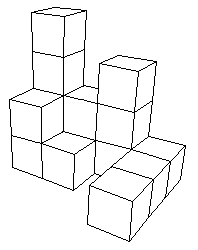
\includegraphics{area}
\end{figure}

Consider the three-dimensional figure above. It is assembled from a number of $1 \times 1 \times 1$ cubes in a 3D grid. If we restrict ourselves to figures that have columns attached to the ``ground'', the figure in the picture can be described by specifying the height of each column:

\begin{verbatim}
4	2	3	1
2	1	0	1
0	0	0	1
\end{verbatim}

The volume of the figure is of course easy to compute, but here we are interested in its bounding surface area, i.e., the number of $1 \times 1$ squares that are visible from the outside (including from below). Write a program that computes this, given the description of a figure.

\section*{Input}
The first line contains two integers $r$ and $k$ ($1 \le r, k \le 50$). Then follow $r$ lines with $k$ integers on each line: the height $h$ ($0 \leq h \leq 50$) of each column.

\section*{Output}
Output a single integer: the bounding surface area of the figure.

\section*{Scoring}
Your solution will be tested on a set of test groups.
To earn points for a group, you must pass all test cases in that group.


\noindent
\begin{tabular}{| l | l | p{12cm} |}
  \hline
  \textbf{Group} & \textbf{Points} & \textbf{Constraints} \\ \hline
  $1$    & $30$       & $h$ is either $0$ or $1$. \\ \hline
  $2$    & $70$       & No additional constraints. \\ \hline
\end{tabular}
